\section{Model}
\label{sec:model}

We formalize the online scheduling problem for Large Language Model (LLM) inference under memory constraints. Unlike traditional scheduling where job sizes are fixed, LLM inference involves \textit{dynamically growing memory demands}: the Key-Value (KV) cache expands continuously as prompts generate output tokens, and the two-phase structure (prefill and decode) creates fundamentally different resource consumption patterns. This dynamic growth, combined with unknown output lengths, distinguishes our problem from classical queueing models. We first introduce the inference process, then describe prompt characteristics, batching rules, system constraints, and performance metrics.

\subsection{Notation}
\label{subsec:notation}
We summarize the key notation used throughout this paper in Table~\ref{tab:notation}.

\begin{table}[h]
\centering
\caption{Summary of Notation}
\label{tab:notation}
\small
\begin{tabular}{cl}
\toprule
\textbf{Symbol} & \textbf{Description} \\
\midrule
$m$ & Number of prompt types \\
$j$ & Index of prompt type, $j \in \{1, \dots, m\}$ \\
$\lambda_j$ & Arrival rate of type-$j$ prompts (Poisson process) \\
$l_j$ & Input length (tokens) of type-$j$ prompts after prefill \\
$l_j'$ & Output length (tokens) of type-$j$ prompts in decode phase \\
$s$ & Stage index: $s = 0$ for prefill, $s \in \{1, \dots, l_j'\}$ for decode \\
$k$ & Segment index in Nested WAIT, $k \in \{1, \dots, m\}$ \\
$b$ & Batch index (iteration count) \\
$n_{js}^t$ & Number of type-$j$ prompts at stage $s$ at time $t$ \\
$n_j$ & Threshold for type-$j$ prompts in WAIT algorithm \\
$n_k$ & Threshold for segment $k$ in Nested WAIT \\
\midrule
$C$ & GPU memory capacity \\
$\mathcal{G}^t$ & Set of prompts with KV cache on GPU at time $t$ \\
$B^t$ & Batch of prompts processed at iteration $t$ ($B^t \subseteq \mathcal{G}^t$) \\
$\tau$ & Iteration time to process a batch \\
$d_0$ & Fixed overhead time per batch iteration \\
$d_1$ & Time cost per unit of KV cache memory \\
\midrule
$M^*$ & Equilibrium memory usage in fluid model \\
$n_j^*$ & Equilibrium number of active type-$j$ prompts \\
$\throughput^*$ & Equilibrium throughput (fluid benchmark) \\
$\Pi$ & Class of admissible scheduling policies \\
\bottomrule
\end{tabular}
\end{table}

\subsection{Prompts and Inference Process}

User queries, called \textit{prompts}, arrive at a single Graphics Processing Unit (GPU) for processing. We focus on maximizing how fully the GPU is used, and our algorithms extend to multi-GPU settings such as pipeline parallelism, where each prompt is processed across different GPUs in different layers of the LLM. When communication costs are negligible, our algorithms apply directly to these settings. 

During inference, each prompt is divided into discrete units called \textit{tokens} during the prefill phase, then generates output text in the decode phase. A token represents a distinct text element, such as a word or subword, and its processing relies on a memory structure called the Key-Value (KV) cache. The KV cache improves inference efficiency by storing the computational history of prior tokens, thus avoiding redundant computations. The cache size increases as tokens are processed, requiring careful memory management to maintain system performance.

% A Central Processing Unit (CPU) with unlimited memory acts as auxiliary storage; however, transferring a token’s KV cache from the CPU to the GPU introduces a delay \( d_s > 0 \) per token.

% \textbf{Prompt Characteristics}: Prompts arrive stochastically and are classified into \( m \) distinct types, indexed by \( j \in \{1, \dots, m\} \). A prompt of type \( j \) has the following properties:
% \[
% \begin{cases}
% \text{a length of } l_j \text{ tokens after completing the prefill phase;} \\
% \text{a length of } l_j + l_j' \text{ tokens after completing the decode phase.}
% \end{cases}
% \]
% We assume that prompts of type \( j \) follow a Poisson process with a rate of \( \lambda_j \).

% \gan{I will add more explanation. The rate $\lambda_j$ comes from the real world inference serving data, and the rate of one type is indeed the sum of rates of many mini types in the real world inference serving data. Or maybe this part should add to the nested WAIT section?}

\textbf{Prompt Characteristics}: Prompts arrive stochastically and are classified into \( m \) distinct types according to their input / output lengths, indexed by \( j \in \{1, \dots, m\} \). We assume that prompts of type \( j \) arrive according to a Poisson process with rate \( \lambda_j \).
% (however, our algorithms and analysis can be extended to more general cases with varying arrival rates, which is left in Appendix \ref{sec:extension}).
Each prompt's memory footprint depends on its processing stage. A prompt of type \( j \) has the following properties:
\begin{equation*}
    \left\{
    \begin{aligned}
        &\text{a length of } l_j \text{ tokens after prefill;}\\
        &\text{a length of } l_j + l_j' \text{ tokens after decode.}
    \end{aligned}
    \right.
\end{equation*}
Therefore, a type-$j$ prompt must undergo one prefill iteration followed by $l_j'$ decode iterations to complete its inference processing. During the prefill phase, the prompt's input context and question are embedded as $l_j$ tokens in a single iteration, consuming a KV cache of size $l_j$ units. In the subsequent decode phase, one output token is generated per iteration, each incurring an additional unit of KV cache memory.

To track processing progress, we define a prompt to be in \textbf{stage $s=0$} if it is about to undergo the prefill phase, and in \textbf{stage $s$} (where $s \in \{1, \dots, l_j'\}$) if it is scheduled to receive its $s$-th output token during the decode phase. Thus, a prompt at stage $s$ occupies memory of size $l_j + s$ units.

Though the total number of different types $m$ can be large (for example, from $1$ to $10000$), our algorithms and their theoretical guarantees exhibit only a weak (logarithmic) dependence on $m$. The analysis relies primarily on the total arrival rate across all types, ensuring that our approach scales efficiently regardless of the number of types.

While our analysis focuses on fixed arrival rates $\lambda_j$, our threshold-based algorithms can be extended to settings with time-varying arrivals by dynamically adjusting thresholds based on the arrival rates (see Section~\ref{sec:extension}).


% The uncertainty of the output length distinguishes our model fundamentally from previous work, such as \cite{jaillet2025onlineschedulingllminference}, which assumes known output lengths. 

\subsection{Batching and Iteration Time}
To use GPU resources efficiently, the GPU processes tasks in \textit{batches}, combining prompts for prefilling and prefilled prompts for decoding. Figure~\ref{fig:batching_example} illustrates this: prompts \( P1 \) and \( P2 \) arrive sequentially and are batched according to their current stage (prefill or decode). The GPU first processes \( P1 \)'s prefill, then \( P2 \)'s prefill. Subsequently, both enter decode, generating one token per iteration in parallel batches. This interleaving of prefill and decode stages improves throughput while managing memory efficiently.


In general, a batch contains two groups: \( n_1 \) prompts in the prefill phase (stage $s=0$), where prompt \( i \) has input length \( l_{j(i)} \) tokens corresponding to its type \( j(i) \) and is processed to initialize its KV cache; and \( n_2 \) prompts in the decode phase, where prompt \( i \) is at stage \( s_i \in \{1, \dots, l_{j(i)}'\} \), having generated \( s_i \) output tokens, with total KV cache size \( l_{j(i)} + s_i \) tokens.


\begin{figure}[h]
    \centering
    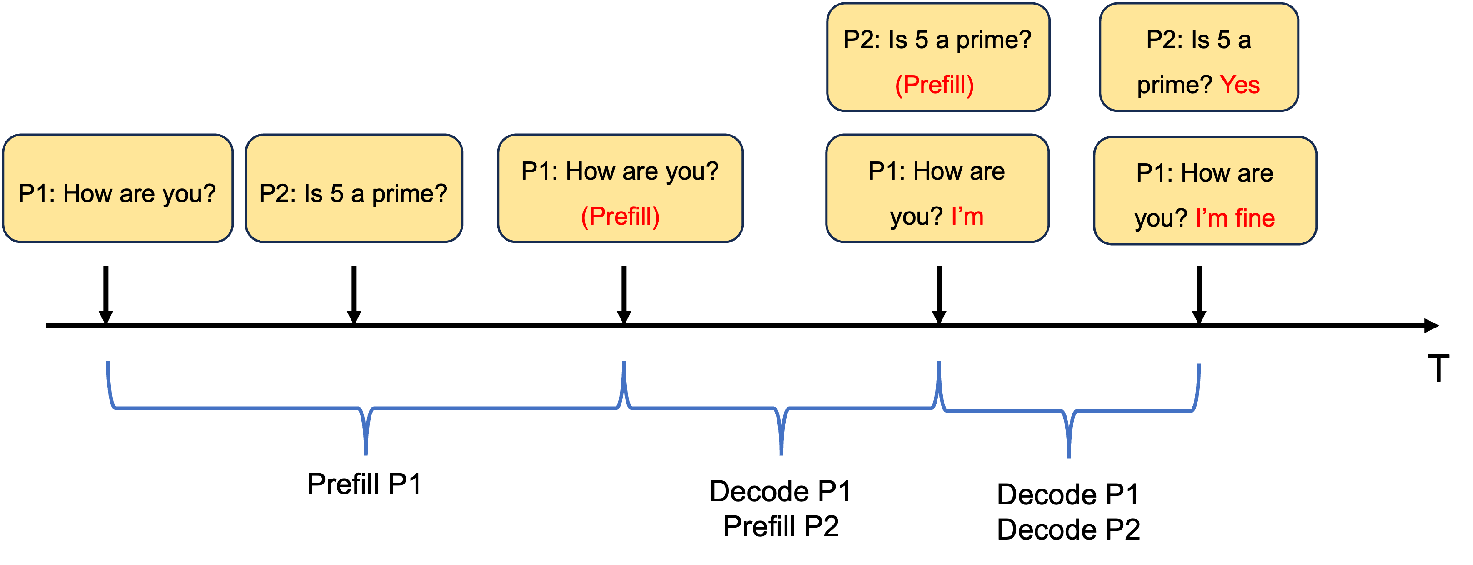
\includegraphics[width=0.6\linewidth]{Experiments_pdf/fig_batching1.pdf}
    \caption{Example of batching and scheduling.}
    \label{fig:batching_example}
\end{figure}

Experiments in \cite{agrawal2023sarathi,kwon2023efficient,zhong2024distserve} show that \textit{iteration time} scales linearly with total KV cache size. We model this as:
\begin{equation}
\label{eq:time_consump}
    \tau = d_0 + d_1 \cdot \underbrace{\left( \sum_{i=1}^{n_1} l_{j(i)} + \sum_{i'=1}^{n_2} (l_{j(i')} + s_{i'}) \right)}_{\text{Total KV cache size}},
\end{equation}
where \( d_0 \) denotes the fixed overhead time associated with processing a batch, and \( d_1 \) represents the time cost per unit of KV cache memory. Equation~\eqref{eq:time_consump} shows that iteration time scales linearly with total KV cache size. The fixed overhead $d_0$ has an important implication: \textit{to maximize throughput, we should use memory as fully as possible}. Larger batches amortize the fixed cost $d_0$ across more prompts, improving efficiency. However, this must be balanced against the memory constraint~\eqref{eq:memory_constraint} to avoid eviction. Figure \ref{fig:inference time} provides a numerical validation of this modeling. We deploy Llama-7B and Llama-13B on a single L20 GPU to test time cost per iteration, using batches consisting of different number of tokens repeated 20 times. The result is highly consistent with our model.

The linear model~\eqref{eq:time_consump} is most accurate when: (i) batches are decode-dominated, as each decode iteration processes one token per prompt and the computational cost is dominated by KV cache memory access; (ii) the system employs prefill-decode disaggregation \citep{zhong2024distserve,patel2024splitwise}, where the decode server handles only decode operations, making Eq.~\eqref{eq:time_consump} exact. In mixed prefill-decode batches, the linear model provides a good approximation when prefill lengths are similar across prompts.

More generally, iteration time can exhibit piecewise linear behavior (e.g., \cite{li2025throughput}), capturing transitions between compute-bound and memory-bound regimes. Our threshold-based algorithms extend naturally to such models, as the key insight---balancing arrivals and completions---remains valid when iteration time scales predictably with batch composition. We adopt the simplified linear model~\eqref{eq:time_consump} for tractability, validated by Figure~\ref{fig:inference time} in the decode-dominated regime.

\begin{figure}
    \centering
    
\includegraphics[width=0.6\linewidth]{Experiments_pdf/inference_time_comparison.pdf}
    \caption{Inference time of Llama-7B and Llama-13B with different number of tokens in the batch on a single L20 GPU}
    \label{fig:inference time}
\end{figure}

\subsection{Memory Constraint and Challenges}

Unlike traditional scheduling where job sizes are fixed, LLM inference faces a unique challenge: prompts occupy memory that \textbf{grows during decode}. Each generated token adds one unit to the prompt's KV cache, causing the memory footprint to expand continuously until completion. This dynamic growth creates eviction risks even when total capacity appears sufficient.

\textbf{Memory Constraint}: At all times $t$, the total KV cache stored on GPU must not exceed capacity $C$:
\begin{equation}
\label{eq:memory_constraint}
\sum_{i \in \mathcal{G}^t} (l_{j(i)} + s^t_i) \le C,
\end{equation}
where $\mathcal{G}^t$ denotes the set of prompts whose KV caches are stored on GPU at time $t$. This includes both prompts actively processed in the current batch $B^t \subseteq \mathcal{G}^t$ and prompts that are preempted but retain their KV caches on GPU. Here $j(i)$ is the type of prompt $i$, and $s^t_i \in \{0, 1, \dots, l_{j(i)}'\}$ is its current stage. Unlike traditional scheduling where job sizes are fixed, the memory footprint $l_{j(i)} + s^t_i$ \textit{grows dynamically} as decode progresses ($s^t_i$ increases each iteration). This dynamic growth creates the risk of \textit{eviction}: if memory becomes insufficient to satisfy the constraint~\eqref{eq:memory_constraint}, ongoing prompts must be removed from the GPU and their KV caches discarded. When eviction is necessary, prompts are removed in \textbf{LIFO order} (most recently admitted prompts are evicted first) until sufficient memory is freed. Evicted prompts lose all accumulated computation and must restart from the prefill phase (stage $s=0$), re-entering the scheduling queue as new arrivals. This creates a vicious cycle: eviction temporarily frees memory, but restarted prompts compete for resources again, potentially triggering further evictions---a phenomenon we call \textit{cascading failure}. The following example illustrates this mechanism.

\begin{example}[Dynamic Memory Growth and Eviction]
\label{ex:memory_growth}
Consider prompts with $(l, l') = (1, 1)$: after prefill, memory is 1 unit; after decode, 2 units. With capacity $C=12$, a stable batch processes 4 prefills (4 units) and 4 decodes (8 units), totaling 12 units.

Now suppose 6 prompts arrive when 3 are decoding (occupying 6 units). Admitting all 6 for prefill fills memory to $6 \times 2 = 12$ units after the 3 existing prompts complete. When 4 new prompts arrive next, prefilling them requires evicting 2 decode prompts to free 4 units. These evicted prompts restart from stage $s=0$, re-entering the queue. The restarted prompts compete with new arrivals, perpetuating the imbalance and triggering repeated evictions---a \textbf{cascading failure}.

This example reveals the core challenge our algorithms target. Even with $C \geq M^*$ (equilibrium memory from Section~\ref{sec:fluid}), poor admission control makes the system unstable. The eviction-restart cycle can persist indefinitely, degrading throughput by 12--25\% (Example~\ref{ex:fcfs_cascade} quantifies this for FCFS).
\end{example}

\paragraph{Core Challenge.}
When output lengths are unknown, optimistic admission risks overflow; pessimistic admission wastes capacity. Our threshold-based algorithms resolve this dilemma by: (i) preventing evictions through controlled admission, (ii) exploiting memory fully via batching, (iii) classifying prompts on-the-fly as they complete decode stages. This approach maintains the system near the load-balanced equilibrium derived in Section~\ref{sec:fluid}, where arrivals match completions and memory use is stable.

\subsection{Performance Metrics}

We optimize \textbf{throughput} (average tokens generated per unit time, counted after prompt completion), subject to constraints on \textbf{latency} (average time from arrival to completion) and \textbf{TTFT} (time to first token, measuring initial user-perceived delay).

\subsection{Optimization Problem and Policy Space}
We formalize the problem as optimizing throughput subject to latency and TTFT constraints over continuous time horizon $[0,T]$:
 

\textbf{Policy Space $\Pi$.} We define the class of admissible scheduling policies $\Pi$. At each decision epoch $t$, a policy $\pi \in \Pi$ observes the system state and makes scheduling decisions subject to the following constraints:

\textit{Information Structure.} The system state at time $t$ includes: (i) the set of all prompts that have arrived by time $t$, along with their input lengths $l_i$; (ii) the current stage $s_i^t$ of each prompt $i$ (i.e., how many output tokens have been generated); (iii) whether each prompt's KV cache is currently stored on GPU. Policies are \textit{non-anticipating}: decisions at time $t$ depend only on information available at or before time $t$. In particular, the output length $l_i'$ of a prompt may be unknown until the prompt completes (generates an end-of-sequence token). This unknown output length is a key challenge addressed by our Nested WAIT algorithm (Section~\ref{sec:nested_wait}).

\textit{Admissible Actions.} At each decision epoch, a policy may:
\begin{enumerate}
    \item \textbf{Admit}: Select a subset of waiting prompts (at stage $s=0$) to enter the system. Admitted prompts wait until included in a batch for prefill.
    \item \textbf{Batch}: Form a batch $B^t$ of prompts to process in the current iteration. After prefill completes, a prompt's KV cache is allocated on GPU.
    \item \textbf{Preempt}: Pause a prompt while retaining its KV cache on GPU. The prompt can resume later without recomputation.
    \item \textbf{Evict}: Remove a prompt's KV cache from GPU to free memory when the constraint~\eqref{eq:memory_constraint} cannot be satisfied. Eviction follows a \textbf{LIFO (Last In, First Out)} policy: the most recently admitted prompts are evicted first. The evicted prompt returns to the waiting queue at stage $s=0$, losing all prior computation.
\end{enumerate}

\textit{Memory Constraint.} At all times, the total KV cache stored on GPU must satisfy the capacity constraint~\eqref{eq:memory_constraint}.

Preemption and eviction are both permitted, but eviction is costly: the evicted prompt re-enters the system as a new arrival and must repeat all processing stages from the beginning. Our WAIT algorithms are designed to \textit{prevent eviction} by controlling admission through thresholds, thereby avoiding the memory pressure that causes eviction. 
% This formulation
% encapsulates the potential trade-offs between resource efficiency and service quality: without the latency and TTFT constraints, the algorithm may always prioritize the shortest jobs in order to maximize the throughput and the latency of the long jobs can be very large in overloaded systems.

% \subsection{Unique Challenges and Comparison to Prior Work}

% This model poses distinct analytical and operational challenges not addressed by conventional scheduling literature:
% \begin{enumerate}
%     \item \textbf{Dynamic memory growth}: Unlike traditional jobs, prompts exhibit progressively increasing memory usage during decoding, complicating classical static memory allocation methods.
%     \item \textbf{Output length uncertainty}: Unlike Jaillet et al. (2025), which assumes known output lengths, our scenario reflects realistic settings where output predictions are unreliable, thus complicating analysis and batch formation strategies.
%     \item \textbf{Multi-stage process}: Prefill and decode phases differ significantly in computational patterns, necessitating a fluid approximation approach to handle their differing resource demands analytically.
% \end{enumerate}

% To address these challenges, we propose a fluid-based analytical framework and threshold-based policies (Sections~\ref{sec:fluid}-\ref{sec:nested_wait}) explicitly designed to operate efficiently under realistic conditions of output uncertainty and stochastic arrivals. This distinguishes our work analytically and practically from existing literature.
